% \section{Introduction}
This section discusses various modifications to the config NoC that can be implemented to improve the configuration speed of the GrAICore.

\section{Improved packet format}
With the current packet format, we observe that there is a significant overhead when writing and reading data.
For every 32 bits of data we read or write, an overhead of 32 bits is also included.
% We propose a new packet format that lessens the overhead.
We explore new packet formats that reduce overhead.
Instead of fixing only two phits containing the read or write data, we can extend the packet to hold more phits containing the data.
We can do this while keeping only one header.
There are a few constraints, however.
Firstly, since the header only contains information for a single destination cluster, all data phits must be destined to the same destination.
Secondly, the data must be read or written in a sequential manner.
This is because the header can only specify a single (starting) address where it should start writing to or reading from.

\subsection{Length field}
We introduce a length field in the header which indicates how many data phits will follow the header phit.
With this information, all nodes involved in the data communication know, by keeping track of the number of phits, when the packet has finished transferring. 

There are some trade-offs between using smaller or larger packets.
A larger packet size increases the efficiency as each packet carries more payload data while header size remains fixed.
Higher efficiency means an improvement in data throughput.
However, increasing the size of the packet will not always offer a considerable increase in data throughput.

To obtain an approximation of the potential speed gains when transferring \SI{36}{MiB} to the GrAICore, we use \cref{eq:latency}.
The amount of overhead can be calculated with \cref{eq:length_field_overhead}.

\begin{equation}
    d_{\text{overhead}} = \frac{d_{\text{payload}}}{n} \times \frac{d_{\text{header}}}{w_{\text{phit}}}
\label{eq:length_field_overhead}
\end{equation}

\begin{eqexpl}[15mm]
    \item{$n$} maximum number of data phits per packet
    \item{$d_{\text{header}}$} size of the header
\end{eqexpl}

Optimal latency can be achieved by taking the largest value for $n$.
\Cref{tab:length_field_optimal_latency} shows the asymptotes or optima for three different phit widths and are calculated by taking the limit as $n$ approaches infinity.
This results in the overhead being $0$ (i.e., $d_{\text{overhead}} = 0$).

\begin{table}[hbtp]
\centering
\begin{tabular}{@{}ll@{}}
\toprule
\textbf{Phit width} & \textbf{Optimal latency (ms)} \\ \midrule
16        & 23.6                  \\
32        & 11.8                  \\
64        & 5.9                   \\ \bottomrule
\end{tabular}
\caption{The latency that can be reached when having a overhead close to none.}
\label{tab:length_field_optimal_latency}
\end{table}

\Cref{fig:n_vs_latency} shows for three different phit sizes the latency to fill the GrAICore for different $n$.
We observe that the latency decreases exponentially, with the latency plateauing earlier with wider phits.

\begin{figure}
    \centering
    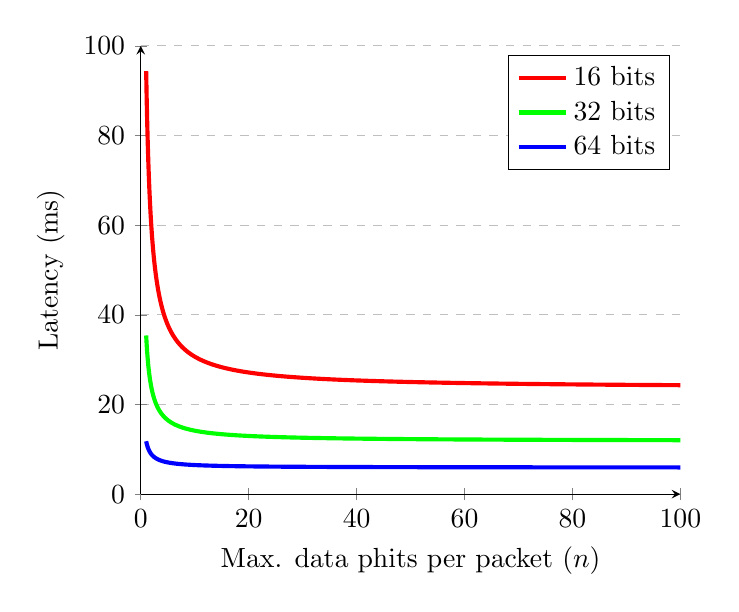
\begin{tikzpicture}
\begin{axis}[
    xmin=0, xmax=100,
    ymin=0, ymax=100,
    axis lines = left,
    xlabel = {Max. data phits per packet ($n$)},
    ylabel = {Latency (ms)},
    ymajorgrids=true,
    grid style=dashed,
]

% 16 bits
\addplot[
    domain=1:100, 
    samples=1000, 
    color=red,
    line width=1.5pt
]
{(((36*1024*1024*8) + ((36*1024*1024*8)/(x) * (16*3)/(16))) / (800000000 * 16)) * 1000};
\addlegendentry{16 bits}
% 32 bits
\addplot[
    domain=1:100, 
    samples=1000, 
    color=green,
    line width=1.5pt
]
{(((36*1024*1024*8) + ((36*1024*1024*8)/(x) * (32*2)/(32))) / (800000000 * 32)) * 1000};
\addlegendentry{32 bits}
% 64 bits
\addplot[
    domain=1:100, 
    samples=1000, 
    color=blue,
    line width=1.5pt
]
{(((36*1024*1024*8) + ((36*1024*1024*8)/(x) * (64*1)/(64))) / (800000000 * 64)) * 1000};
\addlegendentry{64 bits}

\end{axis}
\end{tikzpicture}


    \caption{The trend of latency with increasing $n$.}
    \label{fig:n_vs_latency}
\end{figure}

Note that with $n=15$ the latencies for all three phit widths are close to their optimum.
Since we already use 30 bits for the header information, adding a length field of 4 bits\footnote{$\lceil log_{2}( 15 )\rceil = 4$} requires an additional header phit (i.e., three header phits in total). Similarly, for 32-bit phits, 2 header phits are needed. For 64 bit phits, all information fits within a single header phit.

An example packet format is shown in figure \cref{fig:example_packet_format_length_field} for a phit width of 16 with the length field taking up 4 bits.
An alternative format is to remove two bits of the address field and use those (including the unused bits) for the length field.
With this, we do not require an additional header phit.
Since we have shrunk the address space, we cannot address the SRAM per byte anymore.
Instead, addressing is per 32 bits.
With 4 bits for the length, we can specify a length of up to $2^4 + 1 = 17$.
% We add $1$ since a length of 0 is not practical.
We add $1$ since a header followed by no data phits is not practical.
% It is 17 because a length of 0 is not practical.
This is especially efficient for phit sizes of 32 since all the header information fits within one header phit.
The latency for transferring \SI{36}{MiB} to the GrAICore with a phit width of 32 and length of 17 is computed to be \SI{12.5}{ms}.

\hspace*{0.5em}
\begin{figure}[hbtp]
    \centering
    \begin{adjustbox}{width=0.8\linewidth}
        \begin{bytefield}[
    boxformatting={\centering\ttfamily},
    bitformatting={\ttfamily\small},
    endianness=big,
    bitwidth=2em
]{16}
\bitheader{0, 2, 6, 10, 12, 15} \\

\begin{rightwordgroup}{Header}
    \bitbox{6}[bgcolor=lightcyan]{Address[5:0]} &
    \bitbox{4}[bgcolor=lightred]{Dest. Y} &
    \bitbox{4}[bgcolor=lightorange]{Dest. X} &
    \bitbox{2}[bgcolor=lightgreen]{\scriptsize Packet type} \\

    \bitbox{2}[bgcolor=lightyellow]{\scriptsize Length [1:0]} &
    \bitbox{14}[bgcolor=lightcyan]{Address[19:6]} \\

    \bitbox{14}[bgcolor=lightgray]{Unused} &
    \bitbox{2}[bgcolor=lightyellow]{\scriptsize Length [3:2]}
\end{rightwordgroup} \\

\vspace{-6pt} \\

\begin{rightwordgroup}{Payload}
    \wordbox{1}[bgcolor=lightpurple]{Write data[15:0]} \\
    \wordbox{1}[bgcolor=lightpurple]{Write data[15:0]} \\
    \wordbox[]{1}{$\vdots$} \\[1ex]
    \wordbox{1}[bgcolor=lightpurple]{Write data[15:0]}
\end{rightwordgroup}

\end{bytefield}
    \end{adjustbox}
    \caption{Example packet format with a length field of 4 bits added to the header}
    \label{fig:example_packet_format_length_field}
\end{figure}

\subsection{End bit}
Instead of reserving some bits of the header to indicate the amount of subsequent data phits, we can modify the data phits to include an ``end bit''.
The end bit indicates whether a data phit is the final data phit of a packet.
For this, the header does not need to be changed.
With this approach, the system can send an arbitrary amount of data phits within one packet as it is terminated by the data phit with the end bit set.

In \cref{fig:example_packet_format_end_bit}, we observe that using a phit width of 16, each data phit carries 15 bits of payload data.
Similarly for a phit width of 32 and 64, 31 bits and 63 bits of payload data can be carried, respectively.
However, this specific approach is not practical.
Since the bytes are not aligned, several processing steps have to be performed to align the bytes.
Data alignment is a relatively complex process that requires additional hardware and/or software to be performed.
Consequently, data alignment takes additional time, affecting latency and bandwidth. 

\hspace*{0.5em}
\begin{figure}[hbtp]
    \centering
    \begin{adjustbox}{width=0.8\linewidth}
        \begin{bytefield}[
    boxformatting={\centering\ttfamily},
    bitformatting={\ttfamily\small},
    endianness=big,
    bitwidth=2em
]{16}
\bitheader{0, 2, 6, 10, 12, 15} \\

\begin{rightwordgroup}{Header}
    \bitbox{4}[bgcolor=lightcyan]{Address[3:0]} &
    \bitbox{2}[bgcolor=lightgray]{Unused} &
    \bitbox{4}[bgcolor=lightred]{Dest. Y} &
    \bitbox{4}[bgcolor=lightorange]{Dest. X} &
    \bitbox{2}[bgcolor=lightgreen]{\scriptsize Packet type} \\

    \bitbox{16}[bgcolor=lightcyan]{Address[19:4]}
\end{rightwordgroup} \\

\vspace{-6pt} \\

\begin{rightwordgroup}{Payload}
    \bitbox{1}[bgcolor=lightyellow]{\scriptsize End} &
    \bitbox{15}[bgcolor=lightpurple]{Write data[14:0]} \\
    \bitbox{1}[bgcolor=lightyellow]{\scriptsize End} &
    \bitbox{15}[bgcolor=lightpurple]{Write data[14:0]} \\
    \wordbox[]{1}{$\vdots$} \\[1ex]
    \bitbox{1}[bgcolor=lightyellow]{\scriptsize End} &
    \bitbox{15}[bgcolor=lightpurple]{Write data[14:0]}
\end{rightwordgroup}

\end{bytefield}
    \end{adjustbox}
    \caption{Example packet format with an end bit added to every data phit}
    \label{fig:example_packet_format_end_bit}
\end{figure}

A more efficient way to handle this is to increase the phit width while keeping the payload bytes aligned.
For example, increasing the phit width from 16 to 17 allows 16 bits of payload to be carried by a single data phit.
The remaining bit is the end bit.
Of course, a downside to this is that we require a link width of the same size, effectively meaning that an extra physical wire is required.
This also requires the routers to be modified to accommodate the extra wire.
With this approach, we can calculate the latency with \cref{eq:latency}, using $d_{\text{overhead}}$ as computed with \cref{eq:end_bit_overhead}. 

\begin{equation}
    d_{\text{overhead}} = \frac{d_{\text{payload}}}{w_{phit} - 1} + d_{\text{header}}
\label{eq:end_bit_overhead}
\end{equation}

\Cref{tab:end_bit_latency} show the latency numbers for three different phit widths.
Notice that the latency numbers are similar to the optimal latencies as in the ``length field'' approach. 

\begin{table}[hbtp]
\centering
\begin{tabular}{@{}ll@{}}
\toprule
\textbf{Phit width} & \textbf{Latency (ms)} \\ \midrule
17        & 23.6                  \\
33        & 11.8                  \\
65        & 5.9                   \\ \bottomrule
\end{tabular}
\caption{Best obtainable latencies when using the ``end bit'' approach}
\label{tab:end_bit_latency}
\end{table}

\section{Link width}
With a link width of 16 bits, the config NoC can transfer 16 bits in a single cycle over a link.
Widening the links increases the amount of data that can be transferred in a single cycle.
Physically, this means that the number of wires for each link increases.
Furthermore, the routers need to be enlarged to support the change in link width.
This includes an expansion in buffer size and size of the crossbar switch \cref{TODO}.
These changes will see an increase in the required silicon area and power consumption.

\Cref{tab:latency_bandwidth_phit_width_packet_format,fig:latency_bandwidth_phit_width_packet_format} show for three different phit widths the time it takes to fill the GrAICore and the associated effective bandwidth for the current and the improved packet format.
For the new packet format, we assume that there is overhead.

\begin{table}[hbtp]
\centering
\begin{adjustbox}{width=\linewidth}
\begin{tabular}{@{}lllll@{}}
\toprule
                    & \multicolumn{2}{l}{\textbf{Latency (ms)}} & \multicolumn{2}{l}{\textbf{Effective bandwidth (GiB/s)}} \\ \cmidrule(lr){2-3} \cmidrule(lr){4-5}
\textit{Phit width} & \textit{Current packet format}    & \textit{New packet format}   & \textit{Current packet format}    & \textit{New packet format}   \\ \midrule
16                  & 47.19                    & 23.59               & 0.75                     & 1.49                \\
32                  & 23.59                    & 11.80               & 1.49                     & 2.98                \\
64                  & 11.80                    & 5.90                & 2.98                     & 5.96                \\ \bottomrule
\end{tabular}
\end{adjustbox}
\caption{Latency and effective bandwidth for different phit widths and both packet formats.}
\label{tab:latency_bandwidth_phit_width_packet_format}
\end{table}

\begin{figure}[htbp]
    \centering
    \begin{subfigure}[b]{0.48\textwidth}
        \begin{adjustbox}{width=\linewidth}
            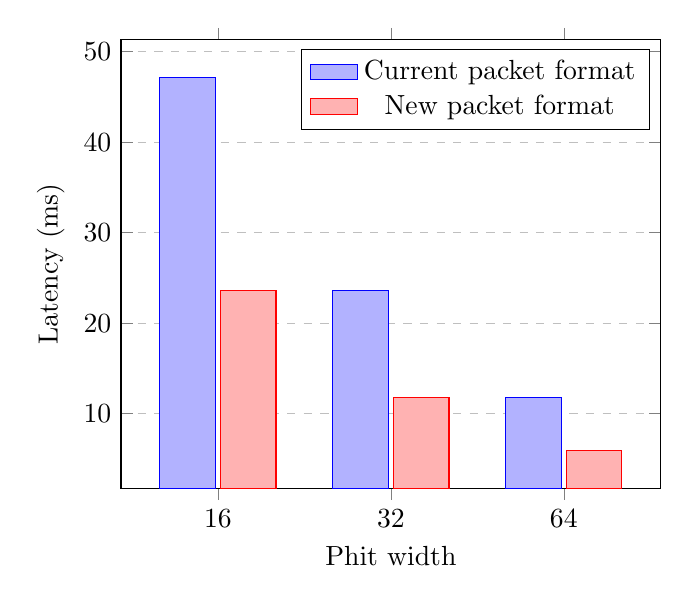
\begin{tikzpicture}
\begin{axis}[
    ylabel=Latency (ms),
    xlabel=Phit width,
    ymajorgrids=true,
    grid style=dashed,
    symbolic x coords={16, 32, 64},
    xtick={16, 32, 64},
    ybar,
    enlarge x limits={abs=35pt},
    bar width=20pt
]

\addplot+[
area legend,
] 
	coordinates {
            (16,47.19)
            (32,23.59)
    	  (64,11.80)
        };
\addplot+[
area legend,
] 
	coordinates {
            (16,23.59)
            (32,11.80)
    	  (64,5.90)
        };
\legend{Current packet format, New packet format}
\end{axis}
\end{tikzpicture}
        \end{adjustbox}
        \caption{Latency}
        % \label{}
    \end{subfigure}
    \hfill
    \begin{subfigure}[b]{0.48\textwidth}
        \begin{adjustbox}{width=\linewidth}
            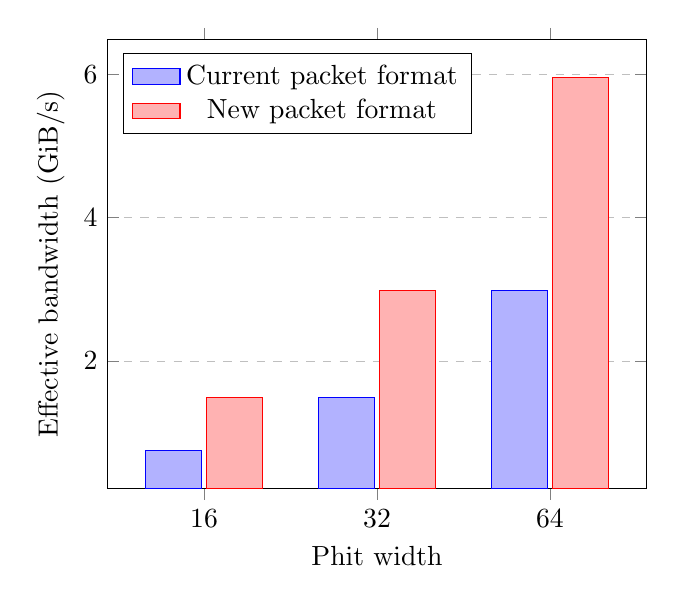
\begin{tikzpicture}
\begin{axis}[
    ylabel=Effective bandwidth (GiB/s),
    xlabel=Phit width,
    ymajorgrids=true,
    grid style=dashed,
    symbolic x coords={16, 32, 64},
    xtick={16, 32, 64},
    ybar,
    enlarge x limits={abs=35pt},
    bar width=20pt,
    legend pos=north west,
]

\addplot+[
area legend,
] 
coordinates {
        (16,0.75)
        (32,1.49)
        (64,2.98)
};
\addplot+[
area legend,
] 
coordinates {
    (16,1.49)
    (32,2.98)
    (64,5.96)
};
\legend{Current packet format, New packet format}
\end{axis}
\end{tikzpicture}
        \end{adjustbox}
        \caption{Effective bandwidth}
        % \label{}
    \end{subfigure}
    \caption[]{For both the old and newly proposed packet formats, the latency is shown for various phit widths}
    \label{fig:latency_bandwidth_phit_width_packet_format}
\end{figure}

\section{Multiple injection points}
The config NoC has a single injection point and only allows for the transmission of a single message at a time.
Thus, when transmitting data from external memory to a neuron core, only a fraction of the NoC's capacity is in use and the remaining part  is left unused.
Also, cores are configured sequentially.
There is a significant potential to improve the utilization of the NoC and parallelism to reduce the configuration time.
We propose to divide the NoC into multiple independent zones.
Each zone is a collection of adjacent clusters including the links between them (example segmentations are illustrated in \cref{fig:segmentation_example}).
Each of the zones is accompanied by a separate interface to the external world, allowing each zone to have data injected into its cores separately and in parallel to other zones.
Having more zones will allow for more parallel data transfers.
To maximize the throughput, the zones should not overlap with each other.
Otherwise, traffic originating from two different sources may cause congestion in the network. 
As a result of this change, the total bandwidth will increase, lowering the end-to-end latency.

We study the effects on performance when introducing multiple injection points.
For three different phit widths and a variety of zones, we compute the latency for sending \SI{36}{MiB} to the GrAICore.
The results are shown in \cref{fig:zones_vs_latency_vs_phit_width} for the old and new packet format.

\begin{figure}[htbp]
    \centering
    \begin{subfigure}[b]{0.48\textwidth}
        \begin{adjustbox}{width=\linewidth}
            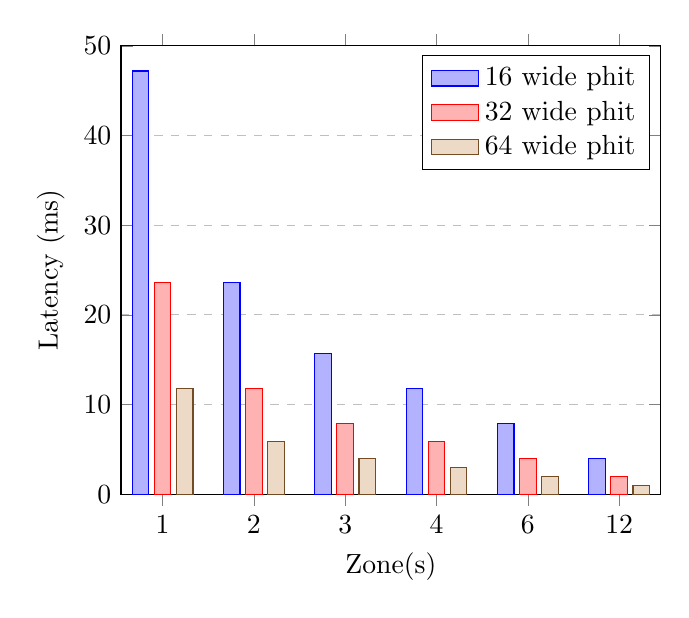
\begin{tikzpicture}
\begin{axis}[
    ylabel=Latency (ms),
    xlabel=Zone(s),
    ymajorgrids=true,
    grid style=dashed,
    ymin=0, ymax=50,
    symbolic x coords={1, 2, 3, 4, 6, 12},
    xtick={1, 2, 3, 4, 6, 12},
    ybar,
    enlarge x limits={abs=15pt},
    bar width=6pt
]

\addplot+[
area legend,
] 
    coordinates {
        (1,47.19)
        (2,23.59)
        (3,15.73)
        (4,11.80)
        (6,7.86)
        (12,3.93)
    };
\addplot+[
area legend,
] 
    coordinates {
        (1,23.59)
        (2,11.80)
        (3,7.86)
        (4,5.90)
        (6,3.93)
        (12,1.97)
    };
\addplot+[
area legend,
] 
    coordinates {
        (1,11.80)
        (2,5.90)
        (3,3.93)
        (4,2.95)
        (6,1.97)
        (12,0.98)
    };
\legend{16 wide phit, 32 wide phit, 64 wide phit}
\end{axis}
\end{tikzpicture}
        \end{adjustbox}
        \caption{Old packet format}
        % \label{}
    \end{subfigure}
    \hfill
    \begin{subfigure}[b]{0.48\textwidth}
        \begin{adjustbox}{width=\linewidth}
            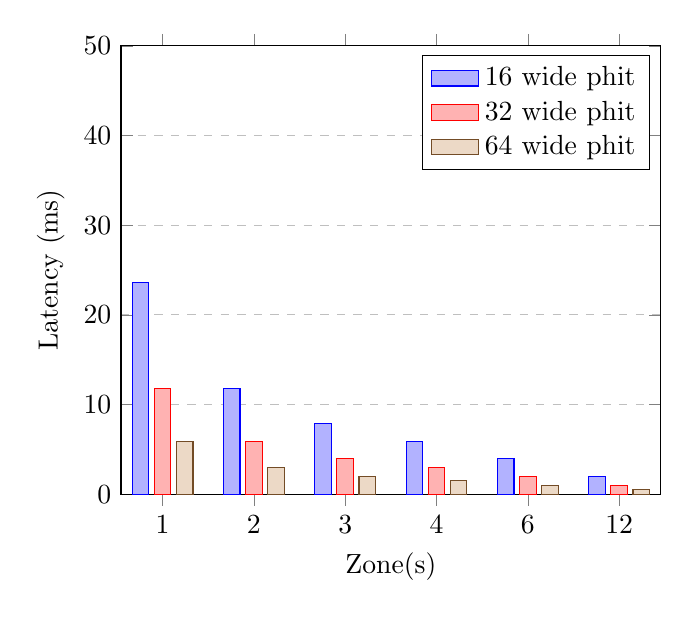
\begin{tikzpicture}
\begin{axis}[
    ylabel=Latency (ms),
    xlabel=Zone(s),
    ymajorgrids=true,
    grid style=dashed,
    ymin=0, ymax=50,
    symbolic x coords={1, 2, 3, 4, 6, 12},
    xtick={1, 2, 3, 4, 6, 12},
    ybar,
    enlarge x limits={abs=15pt},
    bar width=6pt
]

\addplot+[
area legend,
] 
	coordinates {
            (1,23.59)
            (2,11.80)
            (3,7.86)
            (4,5.90)
            (6,3.93)
            (12,1.97)
        };
\addplot+[
area legend,
] 
	coordinates {
            (1,11.80)
            (2,5.90)
            (3,3.93)
            (4,2.95)
            (6,1.97)
            (12,0.98)
        };
\addplot+[
area legend,
] 
	coordinates {
            (1,5.90)
            (2,2.95)
            (3,1.97)
            (4,1.47)
            (6,0.98)
            (12,0.49)
        };
\legend{16 wide phit, 32 wide phit, 64 wide phit}
\end{axis}
\end{tikzpicture}
        \end{adjustbox}
        \caption{New packet format}
        % \label{}
    \end{subfigure}
    \caption[]{The effects of the number of zones and phit width on the latency}
    \label{fig:zones_vs_latency_vs_phit_width}
\end{figure}


Similar to the increase of the phit width, we observe that the number of zones and latency are inversely proportional. While the number of zones and bandwidth are directly proportional.

\begin{figure}[htbp]
    \centering
    \begin{subfigure}[b]{0.48\linewidth}
        \centering
        \begin{adjustbox}{width=0.6\linewidth}
            \begin{tikzpicture}[]
    \draw (-0.5, 0) -- (0, 0);
    \node [diamond, draw, fill=purple] () at (-0.5,0) {};
    
    \draw (0, 0) grid[step=0.5] (5.5,5.5);
    \foreach \x in {0,...,11} {
        \foreach \y in {0,...,11} {
           \node [circle, draw, fill=red] (\x\y) at (0.5*\x,0.5*\y) {};
        }
    }
\end{tikzpicture}
        \end{adjustbox}
        \caption{One zone}
        \label{fig:segmentation_example_1}
    \end{subfigure}
    \hfill
    \begin{subfigure}[b]{0.48\linewidth}
        \centering
        \begin{adjustbox}{width=0.6\linewidth}
            \begin{tikzpicture}[]
    \draw (-0.5, 3) -- (0, 3);
    \node [diamond, draw, fill=purple] () at (-0.5,3) {};
    
    \draw (-0.5, 0) -- (0, 0);
    \node [diamond, draw, fill=purple] () at (-0.5,0) {};
    
    \draw (0, 0) grid[step=0.5] (5.5,5.5);
    \foreach \x in {0,...,11} {
        \foreach \y in {0,...,5}  {
           \node [circle, draw, fill=red] (\x\y) at (0.5*\x,0.5*\y) {};
        }
        \foreach \y in {6,...,11} {
           \node [circle, draw, fill=blue] (\x\y) at (0.5*\x,0.5*\y) {};
        }
    }
\end{tikzpicture}

        \end{adjustbox}
        \caption{Two zones}
        \label{fig:segmentation_example_2}
    \end{subfigure}
    \\ \vspace{1.5em}
    \begin{subfigure}[b]{0.48\linewidth}
        \centering
        \begin{adjustbox}{width=0.6\linewidth}
            \begin{tikzpicture}[]
    \draw (-0.5, 4) -- (0, 4);
    \node [diamond, draw, fill=purple] () at (-0.5,4) {};
    
    \draw (-0.5, 2) -- (0, 2);
    \node [diamond, draw, fill=purple] () at (-0.5,2) {};
    
    \draw (-0.5, 0) -- (0, 0);
    \node [diamond, draw, fill=purple] () at (-0.5,0) {};
    
    \draw (0, 0) grid[step=0.5] (5.5,5.5);
    \foreach \x in {0,...,11} {
        \foreach \y in {0,...,3}  {
           \node [circle, draw, fill=red] (\x\y) at (0.5*\x,0.5*\y) {};
        }
        \foreach \y in {4,...,7} {
           \node [circle, draw, fill=blue] (\x\y) at (0.5*\x,0.5*\y) {};
        }
        \foreach \y in {8,...,11} {
           \node [circle, draw, fill=green] (\x\y) at (0.5*\x,0.5*\y) {};
        }
    }
\end{tikzpicture}

        \end{adjustbox}
        \caption{Three zones}
        \label{fig:segmentation_example_3}
    \end{subfigure}
    \hfill
    \begin{subfigure}[b]{0.48\linewidth}
        \centering
        \begin{adjustbox}{width=0.6\linewidth}
            \begin{tikzpicture}[]
    \draw (-0.5, 4.5) -- (0, 4.5);
    \node [diamond, draw, fill=purple] () at (-0.5,4.5) {};
    
    \draw (-0.5, 3) -- (0, 3);
    \node [diamond, draw, fill=purple] () at (-0.5,3) {};
    
    \draw (-0.5, 1.5) -- (0, 1.5);
    \node [diamond, draw, fill=purple] () at (-0.5,1.5) {};
    
    \draw (-0.5, 0) -- (0, 0);
    \node [diamond, draw, fill=purple] () at (-0.5,0) {};
    
    \draw (0, 0) grid[step=0.5] (5.5,5.5);
    \foreach \x in {0,...,11} {
        \foreach \y in {0,...,2}  {
           \node [circle, draw, fill=red] (\x\y) at (0.5*\x,0.5*\y) {};
        }
        \foreach \y in {3,...,5} {
           \node [circle, draw, fill=blue] (\x\y) at (0.5*\x,0.5*\y) {};
        }
        \foreach \y in {6,...,8} {
           \node [circle, draw, fill=green] (\x\y) at (0.5*\x,0.5*\y) {};
        }
        \foreach \y in {9,...,11} {
           \node [circle, draw, fill=yellow] (\x\y) at (0.5*\x,0.5*\y) {};
        }
    }
\end{tikzpicture}
        \end{adjustbox}
        \caption{Four zones}
        \label{fig:segmentation_example_4}
    \end{subfigure}
    \caption{
    Example segmentation of the config NoC into multiple zones.
    A zone is a set of nodes (circle shapes) and is illustrated by a distinct color.
    The diamond shapes show the unique injection sources for each zone.
    }
    \label{fig:segmentation_example}
\end{figure}
